\begin{frame}
\frametitle{Linear regression: maximum likelihood}
A simple way to do regression is by:
\begin{align*}
f({\bf x}_*) = {\bf w}^T {\bf x}_*
\end{align*}
Assuming Gaussian noise on ${\bf y}$, the ML estimate of ${\bf w}$ is by:
\begin{align*}
\hat{\bf w} = ({\bf X}^T{\bf X})^{-1}{\bf X}^T {\bf y}
\end{align*}
where
\begin{align*}
{\bf X} = \begin{pmatrix}{\bf x}_1 & {\bf x}_2 & \hdots & {\bf x}_n\end{pmatrix}^T \text{, and }
{\bf y} = \begin{pmatrix}y_1 & y_2 & \hdots y_n\end{pmatrix}^T
\end{align*}
Model has $p$ parameters to estimate.\par
Number of observations is $n$ (number of targets).\par
Usually needs dimensionality reduction, with (eg) SVD.
\end{frame}

\begin{frame}
\frametitle{Linear regression: maximum posterior}
We may have prior knowledge about various distributions:
\begin{align*}
p(y_* | {\bf x}_*, {\bf w}) = & \mathcal{N}({\bf w}^T{\bf x}_*, \sigma^2)\cr
p({\bf w}) = & \mathcal{N}({\bf 0},\boldsymbol\Sigma_0)\cr
\end{align*}
Therefore,
\begin{align*}
p({\bf w}|{\bf y},{\bf X})  = & \mathcal{N}(\sigma^{-2}{\bf B}^{-1}{\bf X}^T{\bf y},{\bf B}^{-1}) \text{, where } {\bf B} = \sigma^{-2}{\bf X}^T{\bf X} + \boldsymbol\Sigma_0^{-1}
\end{align*}

Maximum a posteriori (MAP) estimate of ${\bf w}$ is by:
\begin{align*}
\hat{\bf w} = \sigma^{-2}{\bf B}^{-1}{\bf X}^T{\bf y} \text{, where } {\bf B} = \sigma^{-2}{\bf X}^T{\bf X} + \boldsymbol\Sigma_0^{-1}
\end{align*}
\end{frame}

\begin{frame}
\frametitle{Linear regression: Bayesian}
We may have prior knowledge about various distributions:
\begin{align*}
p(y_* | {\bf x}_*, {\bf w}) = & \mathcal{N}({\bf w}^T{\bf x}_*, \sigma^2)\cr
p({\bf w}) = & \mathcal{N}({\bf 0},\boldsymbol\Sigma_0)\cr
\end{align*}
Therefore,
\begin{align*}
p({\bf w}|{\bf y},{\bf X})  = & \mathcal{N}(\sigma^{-2}{\bf B}^{-1}{\bf X}^T{\bf y},{\bf B}^{-1}) \text{, where } {\bf B} = \sigma^{-2}{\bf X}^T{\bf X} + \boldsymbol\Sigma_0^{-1}
\end{align*}
Predictions are made by integrating out the uncertainty of the weights, rather than estimating them:
\begin{align*}
p(y_* | {\bf x}_*, {\bf y}, {\bf X}) = & \int_{\bf w} p(y_* | {\bf x}_*, {\bf w}) p({\bf w}|{\bf y},{\bf X}) d{\bf w}\cr
                                     = & \mathcal{N}(\sigma^{-2} {\bf x}_*^T {\bf B}^{-1} {\bf X}^T {\bf y}, {\bf x}_*^T{\bf B}^{-1}{\bf x}_*)
\end{align*}
Estimated parameters may be $\sigma^2$, and parameters encoding $\boldsymbol\Sigma_0$.
\end{frame}

\begin{frame}
\frametitle{Kernel methods: Woodbury matrix identity}
\begin{align*}
{\bf B}^{-1} = & \left(\sigma^{-2}{\bf X}^T{\bf X} + \boldsymbol\Sigma_0^{-1}\right)^{-1} & \text{ invert a } p \times p \text{ matrix}\\
             = & \boldsymbol\Sigma_0 - \boldsymbol\Sigma_0 {\bf X}^T({\bf I}\sigma^2 + {\bf X} \boldsymbol\Sigma_0 {\bf X}^T)^{-1} {\bf X} \boldsymbol\Sigma_0 & \text{ invert an } n \times n \text{ matrix}
\end{align*}

\vspace{0.25cm}
\begin{tiny}
Wikipedia contributors, ``Woodbury matrix identity,'' Wikipedia, The Free Encyclopedia, \url{http://en.wikipedia.org/w/index.php?title=Woodbury\_matrix\_identity\&oldid=638370219} (accessed April 1, 2015).\par
$({\bf A}+{\bf U}{\bf C}{\bf V})^{-1} = {\bf A}^{-1} - {\bf A}^{-1} {\bf U}({\bf C}^{-1} + {\bf V}{\bf A}^{-1}{\bf U})^{-1}{\bf V}{\bf A}^{-1}$.\par
\end{tiny}
\end{frame}

\begin{frame}
\frametitle{Kernel methods: Gaussian process regression}
The predicted distribution is:
\begin{align*}
p(y_*|{\bf x}_*,{\bf y},{\bf X}) = &\mathcal{N}({\bf k}^T{\bf C}^{-1} {\bf y},c - {\bf k}^T {\bf C}^{-1} {\bf k})
\end{align*}
where:
\begin{align*}
{\bf C} = & {\bf X} \boldsymbol\Sigma_0 {\bf X}^T + {\bf I}\sigma^2\\
{\bf k} = & {\bf X} \boldsymbol\Sigma_0 {\bf x}_*\\
c = & {\bf x}_*^T \boldsymbol\Sigma_0 {\bf x}_* + \sigma^2
\end{align*}
\end{frame}

\begin{frame}
\frametitle{Kernel methods: nonlinear methods}
%\begin{columns}[c]
%\column{0.5\textwidth}
Sometimes, we want alternatives to ${\bf C} = {\bf X} \boldsymbol\Sigma_0 {\bf X}^T + {\bf I}\sigma^2$.\par
Nonlinearity is achieved by replacing the matrix ${\bf K} = {\bf X} \boldsymbol\Sigma_0 {\bf X}^T$ with some function of the data that gives a positive definite matrix encoding similarities.\par
eg
\begin{align*}
k({\bf x}_i,{\bf x}_j) = \theta_1 + \theta_2 {\bf x}_i \cdot {\bf x_j} + \theta_3 \exp\left(-\frac{||{\bf x}_i - {\bf x_j}||^2}{2 \theta_4^2}\right)
\end{align*}

Hyper-parameters $\theta_1$ to $\theta_4$ can be optimised in a number of ways.\par
%\column{0.5\textwidth}
%Examples include:
%\begin{itemize}
%\item Linear: $k({\bf x}_i,{\bf x}_j) = {\bf x}_i \cdot {\bf x}_k$
%\item 
%\end{itemize}
%\includegraphics[width=.75\textwidth]{nonlinear_kernels}
%\end{columns}
\end{frame}

\begin{frame}
\frametitle{Kernel methods: nonlinear methods}
\begin{columns}[cc]
\column{0.6\textwidth}
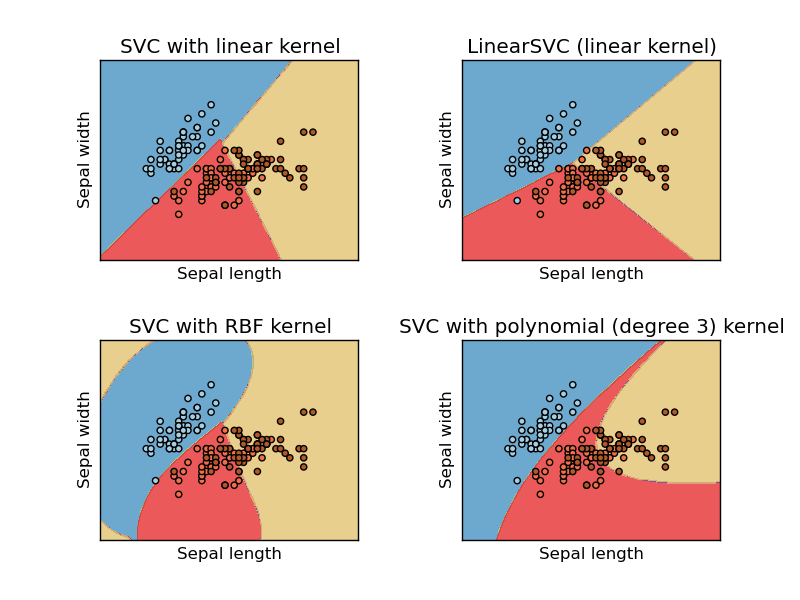
\includegraphics[width=\textwidth]{sklearn_material/plot_iris_0012.png}
\column{0.4\textwidth} Non-linear methods are useful in low-dimension
to adapt the shape of decision boundaries.
\end{columns}
For large $p$, small $n$ problems, nonlinear methods do not seem to help much.\par
Nonlinearity also reduces interpretability.
\end{frame}

\begin{frame}
\frametitle{Probabilistic discriminative models}
\begin{columns}[c]
\column{0.5\textwidth}
\begin{block}
{\bf Regression}\par
Continuous targets:
\begin{align*}
y \in \mathcal{R}
\end{align*}
Usually assume a Gaussian distribution:
\begin{align*}
p(&y|{\bf x},{\bf w}) =\\
& \mathcal{N}(f({\bf x},{\bf w}),\sigma^2)
\end{align*}
where $\sigma^2$ is a variance.\par
\end{block}
\column{0.5\textwidth}
\begin{block}
{\bf Binary Classification}\par
Categorical targets:
\begin{align*}
y \in \{0,1\}
\end{align*}
Usually assume a binomial distribution:
\begin{align*}
p(&y|{\bf x},{\bf w}) =\\
& \sigma(f({\bf x},{\bf w}))^{y} (1 - \sigma(f({\bf x},{\bf w})))^{1-y}
\end{align*}
where $\sigma$ is a squashing function.\par
\end{block}
\end{columns}
\end{frame}

\begin{frame}
\frametitle{Probabilistic discriminative models}
\begin{columns}[c]
\column{0.5\textwidth}
For binary classification:
\begin{align*}
p(y_*=1|{\bf x}_*,{\bf w}) = \sigma(f({\bf x}_*,{\bf w}))
\end{align*}
where $\sigma$ is some squashing function, eg:
\begin{itemize}
\item Logistic sigmoid function (inverse of Logit).
\item Normal CDF (inverse of Probit).
\end{itemize}
\column{0.5\textwidth}
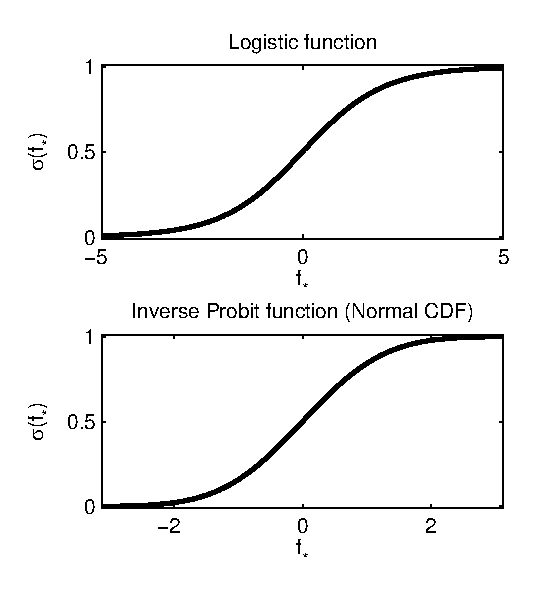
\includegraphics[width=.75\textwidth]{squashing}
\end{columns}
\end{frame}

\begin{frame}
\frametitle{Probabilistic discriminative models}
\begin{columns}[c]
\column{0.5\textwidth}
Integrating over the uncertainty of the separating hyperplane allows probabilistic predictions further from the training data.\par
This is not usually done for methods such as the relevance-vector machine (RVM).\par
\vspace{0.25cm}
\begin{tiny}
Rasmussen, Carl Edward, and Joaquin Quinonero-Candela. ``Healing the relevance vector machine through augmentation.'' In Proceedings of the 22nd international conference on Machine learning, pp. 689-696. ACM, 2005.\par
\end{tiny}
\column{0.5\textwidth}
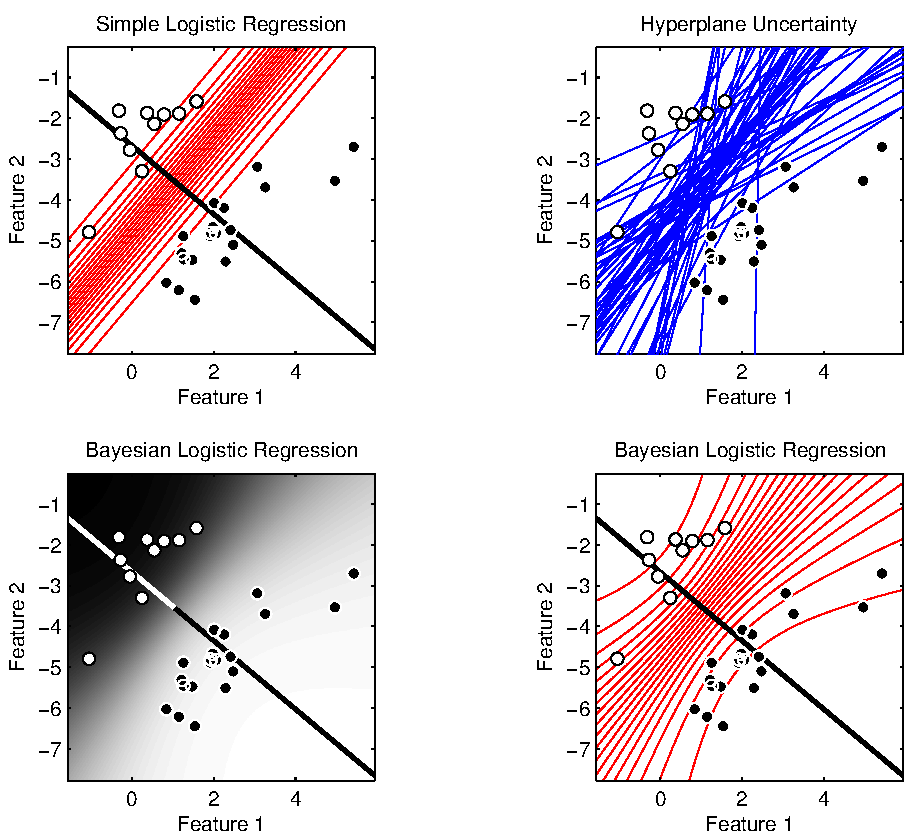
\includegraphics[width=\textwidth]{logistic_regr}
\end{columns}
\end{frame}

\begin{frame}
\frametitle{Probabilistic discriminative models}
Making probabilistic predictions involves:
\begin{enumerate}
\item Computing the distribution of a latent variable corresponding to the test data (cf regression):
\begin{align*}
p(f_* | {\bf x}_*, {\bf y}, {\bf X}) = & \int_{\bf f} p(f_* | {\bf x}_*, {\bf f}) p({\bf f}|{\bf y},{\bf X}) d{\bf f}
\end{align*}
\item Using this distribution to give a probabilistic prediction:
\begin{align*}
P(y_*=1|{\bf x}_*,{\bf y},{\bf X}) = \int_{f_*} \sigma(f_*) p(f_*|{\bf x}_*,{\bf y},{\bf X}) df_*
\end{align*}
\end{enumerate}
Unfortunately, these integrals are analytically intractable, so approximations are needed.\par
\end{frame}

\begin{frame}
\frametitle{Probabilistic discriminative models}
Approximate methods for probabilistic classification include:
\begin{itemize}
\item {\bf The Laplace Approximation} (LA).  Fastest, but less accurate.
\item {\bf Expectation Propagation} (EP).  More accurate than the Laplace approximation, but slightly slower.
\item {\bf MCMC} methods. The ``gold standard'', but very slow to draw lots of random samples.
\end{itemize}
\vspace{0.25cm}
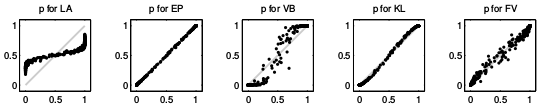
\includegraphics[width=\textwidth]{nickisch_figure}
\begin{tiny}
Nickisch, Hannes, and Carl Edward Rasmussen. ``Approximations for Binary Gaussian Process Classification.'' Journal of Machine Learning Research 9 (2008): 2035-2078.\par
\end{tiny}
\end{frame}



\begin{frame}
\frametitle{Discriminative models for classification}
\begin{columns}[c]
\column{0.5\textwidth}
\begin{align*}
t = \sigma(f({\bf x}_*)) 
\end{align*}
where $\sigma$ is some squashing function, eg:
\begin{itemize}
%\item Heaviside step function.
\item Logistic function (inverse of Logit).
\item Normal CDF (inverse of Probit).
\item Hinge loss (support vector machines)
\end{itemize}
\column{0.5\textwidth}
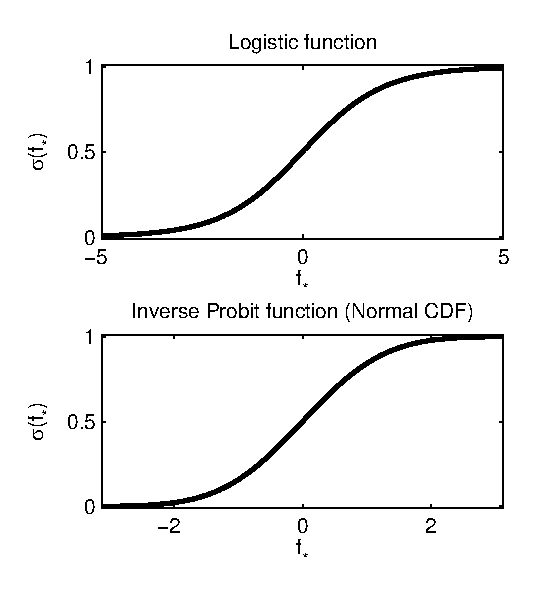
\includegraphics[width=.75\textwidth]{squashing}

%\textbf{Bertrand: maybe a distinction should be introduced here between the decision function (typically the sign function) and the loss function used for training.}

\end{columns}
\end{frame}

\begin{frame}
\frametitle{Discriminative models for classification: convexity}
%
%Convex losses yield well-defined solution and are preferred.
%
\begin{align*}
\text{(M-estimators framework)} \; \; \text{min}_{\mathbf{w}} \; \sum_{i=1}^n \mathcal{L}(y_i,\mathbf{X_i},\mathbf{w}) + \alpha \mathcal{R} (\mathbf{w})
\end{align*}
%
\begin{columns}[c]
\column{.6\textwidth}
\begin{itemize}
\item $\mathcal{L}$ is the loss function (hinge, logistic, quadratic...)
\item $\mathcal{R}$ is the regularizer (typically a norm on $\mathbf{w}$)
\item $\alpha > 0$ balances the two terms
\end{itemize}
$\mathcal{L}$ and $\mathcal{R}$ convex $\rightarrow$ unique minimizer (SVMs, $\ell_2$-logistic, $\ell_1$-logistic).
\column{.4\textwidth}
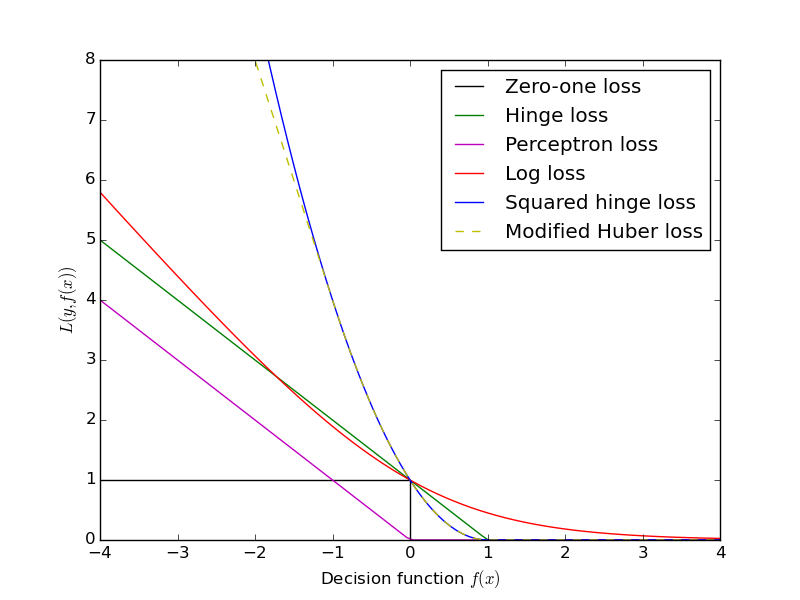
\includegraphics[width=1.2\textwidth]{sklearn_material/plot_sgd_loss_functions_001.png}
\end{columns}
\end{frame}


\begin{frame}
\frametitle{Support vector classification}
\begin{columns}[c]
\column{0.5\textwidth} SVMs are reasonably fast, accurate and easy to
tune ($C=10^3$ is a good default, no dramatic failure).\\ % Doesn't this epend on how the features are scaled?

Multi-class: One-versus-one, One-versus all.

\par
%Targets are ${\bf t} \in \{-1,1\}$.\\
%Solves a quadratic programming problem
%\begin{align*}
%\hat{\boldsymbol\alpha} = \argmin_{\boldsymbol\alpha} \tfrac{1}{2} {\boldsymbol\alpha}^T {\bf H}{\boldsymbol\alpha} - \sum_{i=1}^n \alpha_i,\\
%\text{subject to }
%{\bf t}^T{\boldsymbol\alpha} = 0 \text{ and }
%0 \le \alpha_i \le C\\
%\text{where }
%{\bf H} = \diag({\bf t}) {\bf X}{\bf X}^T \diag({\bf t})
%\end{align*}
%Binary prediction is by:
%\begin{align*}
%t_* = sgn(\sum_{i=1}^N t_i \alpha_i {\bf x}_i {\bf x}_*^T + b)
%\end{align*}
%where $b$ is a bias term.
\column{0.5\textwidth}
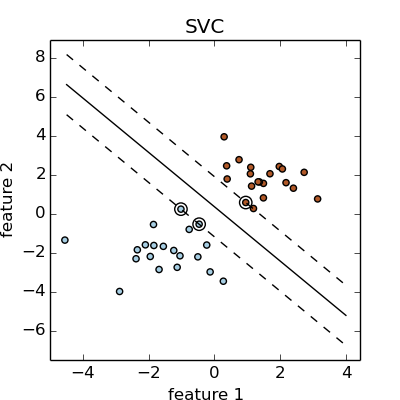
\includegraphics[width=\textwidth]{sklearn_material/plot_separating_hyperplane_0011.png}
\end{columns}
\end{frame}

\begin{frame}
\frametitle{Convex methods in regression}

(M-estimators framework)

\begin{align*}
\text{min}_{\mathbf{w}} \; \sum_{i=1}^n \mathcal{L}(y_i,\mathbf{X_i},\mathbf{w}) + \alpha \mathcal{R} (\mathbf{w})
\end{align*}


\begin{columns}
\column{0.65\textwidth}
\begin{itemize}
\item $\mathcal{L}$ is the loss function (quadratic, $\varepsilon-$insensitive, Huber)
\item $\mathcal{R}$ is the regularizer (typically a norm on $\mathbf{w}$)
\item $\alpha > 0$ balances the two terms
\end{itemize}
$\mathcal{L}$ and $\mathcal{R}$ convex $\rightarrow$ unique minimizer (Ridge, Lasso, Elastic Net regression).
\column{0.35\textwidth}
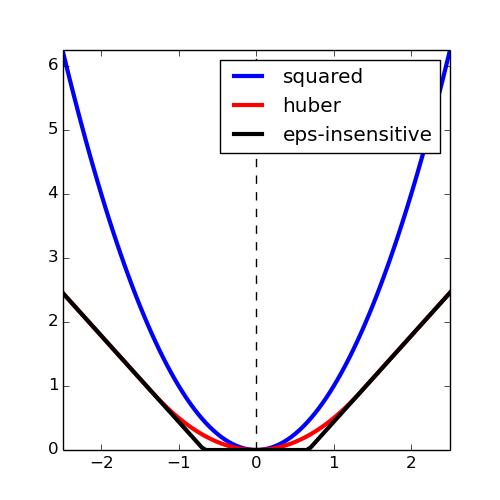
\includegraphics[width=\textwidth]{sklearn_material/losses.png}

\end{columns}
\end{frame}


\begin{frame}
\frametitle{Ridge Regression}

\begin{align*}
\text{min}_{\mathbf{w}} \; \frac{1}{2n} \sum_{i=1}^n \|y_i - \mathbf{X_i}\mathbf{w}\|^2 + \alpha \|\mathbf{w}\|^2
\end{align*}


\begin{columns}
\column{0.4\textwidth}
\begin{itemize}
\item Fast, closed-form
\item Non-sparse solution
\item $\alpha > 0$ can be set by generalized cross-validation
\end{itemize}
\column{0.6\textwidth}
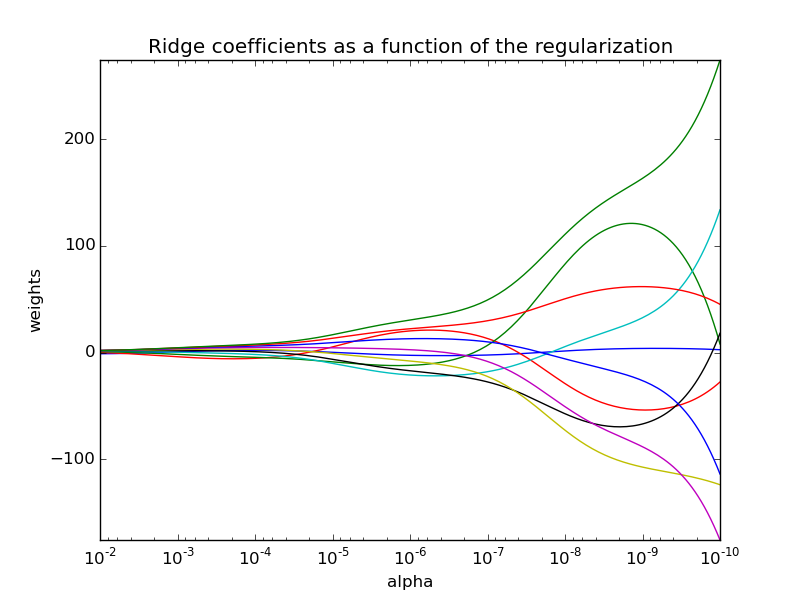
\includegraphics[width=\textwidth]{sklearn_material/plot_ridge_path_0011.png}

\end{columns}
\end{frame}


\begin{frame}
\frametitle{Lasso Regression}

\begin{align*}
\text{min}_{\mathbf{w}} \; \frac{1}{2n} \sum_{i=1}^n \|y_i - \mathbf{X_i}\mathbf{w}\|^2 + \alpha \|\mathbf{w}\|_1
\end{align*}

\begin{columns}
\column{0.4\textwidth}
\begin{itemize}
\item Solved by LARS, coordinate descent or proximal
\item Sparse solution
\item $\alpha > 0$ harder to tune
\end{itemize}
\column{0.6\textwidth}
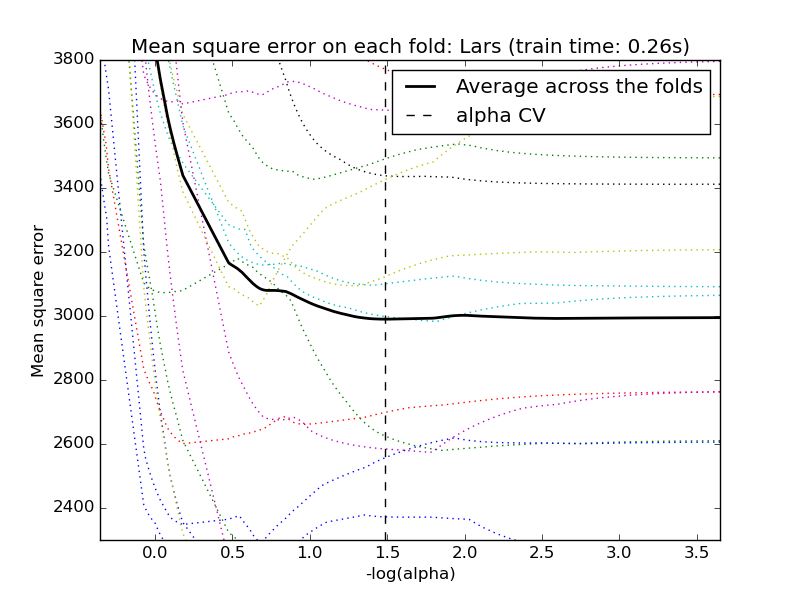
\includegraphics[width=\textwidth]{sklearn_material/plot_lasso_model_selection_003.png}

\end{columns}
\end{frame}


\begin{frame}
\frametitle{Elastic Net Regression}

\begin{align*}
\text{min}_{\mathbf{w}} \; \frac{1}{2n} \sum_{i=1}^n \|y_i - \mathbf{X_i}\mathbf{w}\|^2 + \alpha \left( \rho \|\mathbf{w}\|_1 + (1-\rho) \|\mathbf{w}\|^2 \right) 
\end{align*}

\begin{columns}
\column{0.4\textwidth}
\begin{itemize}
\item Solved by coordinate descent or proximal
\item Sparse solution
\item $\alpha > 0$ and $\rho \in [0,1]$ harder to tune
\end{itemize}
\column{0.6\textwidth}
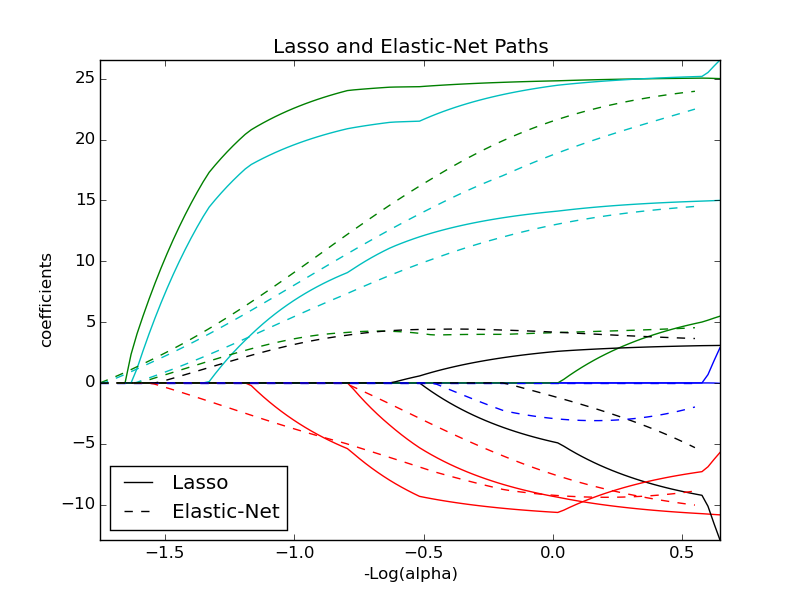
\includegraphics[width=\textwidth]{sklearn_material/plot_lasso_coordinate_descent_path_0011.png}

\end{columns}
\end{frame}
